% This file contains CHAPTER THREE

\chapter{Balanced NUCOMP}\label{cha:nucomp} In Chapter~\ref{cha:bg}, arithmetic
in the divisor class group of a hyperelliptic curve, expressed in terms of
polynomial arithmetic, was described by Cantor's Addition
(Algorithm~\ref{alg:cantoradd}) for ramified models and adapted to Balanced
Addition (Algorithm~\ref{alg:baladd}) for split models. Various improvements and
extensions to Cantor's algorithm have been proposed, including an adaptation of
Shank's NUCOMP algorithm~\cite{ShanksNUCOMP} for composing binary quadratic
forms~\cite{jacobson_nucomp_2002}. The main idea behind NUCOMP is that instead
of composing two divisors directly and then reducing to find an equivalent
reduced divisor, a type of reduction is applied part way through the
composition, so that when the composition is finished the result is almost
always reduced.  The effect is that the sizes of the intermediate operands are
reduced and the intermediate Mumford representations are not computed,
resulting in better performance in most cases. Improvements to NUCOMP have been
proposed, most recently the work of~\cite{ImbJac13:amc}, where best practices
for computing Cantor's algorithm and NUCOMP  for divisor arithmetic on
hyperelliptic curves are empirically investigated.  NUCOMP has also been
proposed for arithmetic in the infrastructure of a split model
curve~\cite{jacobson_fast_2007}. Although the balanced divisor setting for
divisor class group arithmetic on split models due to Galbraith et.\ al.
\cite{Galbraith_balanced_2008,Morales_balanced_2009} is in some ways similar to
the infrastructure, NUCOMP has yet to be applied explicitly to that setting.

The novel contribution of this chapter is an adaptation of NUCOMP for divisor
class group arithmetic on split model hyperelliptic curves that uses the
balanced divisor framework. Efficient algorithmic practices from previous work
in the ramified model setting are incorporated and new balanced setting-specific
improvements that further enhance practical performance are introduced.
Specifically, the new version of NUCOMP includes the following improvements over
\cite{jacobson_fast_2007}:
\begin{itemize}
    \item describes for the first time exactly how to use NUCOMP in the
    framework of balanced divisors, including explicit computations of the
    required balancing coefficients; (Section~\ref{sec:balNUCOMP}),
    \item introduces a novel normalization of divisors in order to eliminate the
    extra adjustment step required in \cite{jacobson_fast_2007} for frequent
    inputs when the genus of the hyperelliptic curve is odd, so that in all
    cases frequent inputs require no extra reduction nor adjustment steps;
    (Section~\ref{sec:negreduced}),
    \item uses certain aspects of NUCOMP to compute one adjustment step almost
    for free in some cases. (Section~\ref{sec:eliminateadj}). 
\end{itemize} 
Numerical results that demonstrate the efficiency gains realized from the new
version of NUCOMP as compared with the previous best balanced divisor class
group arithmetic based on Cantor's algorithm and Magma's built-in arithmetic are
presented, showing that NUCOMP is the method of choice for all but the smallest
genera. Moreover, the novel NUCOMP algorithm for split model divisor class
arithmetic introduced in this chapter reduces the complexity of explicit
formulas over split model genus 2 and 3 hyperelliptic curves discussed in
Chapters~\ref{cha:g2} and~\ref{cha:g3} respectively.

The rest of the chapter is organized as follows.  In
Section~\ref{sec:improvements}, improvements to Cantor's Addition algorithm are
discussed and improved divisor class addition algorithms for ramified and split
model hyperelliptic curves are presented. In Section~\ref{sec:NUCOMP}, a NUCOMP
based algorithm for computing divisor class arithmetic over ramified curves is
described using all applicable improvements from Section~\ref{sec:improvements}.
In Section~\ref{sec:balNUCOMP} the main contribution of this chapter, a novel
adaptation of NUCOMP, denoted \emph{Balanced NUCOMP}, for computing divisor
class arithmetic in the balanced setting of a split hyperelliptic curve is
presented along with numerical results comparing the new algorithm with the
previous best balanced addition algorithm.

\section{Improvements to Addition Algorithms}\label{sec:improvements} In this
section, formulations of Cantor's and Balanced addition algorithms are presented
that include a variety of practical improvements taken from the most recent work
on this topic~\cite{ImbJac13:amc}. First, techniques for improving the
efficiency of both Cantor's and Balanced addition
(Algorithms~\ref{alg:cantoradd} and~\ref{alg:baladd}) are described. Then the
improved Cantor's addition algorithm, along with a version specialized to
doubling for the ramified setting is presented. Finally, a computationally
beneficial normalization of the $v$ polynomial for the balanced setting is given
and the resulting improved Balanced addition and doubling algorithms described.

\subsection{General Techniques}\label{sec:polytechniques} There are two main
techniques used in the improvement of Cantor's Addition in~\cite{ImbJac13:amc}:
optimization for the most frequently-occurring input and the use of Tenner's
algorithm for reduction, which requires a revised Mumford representation that
uses a computationally useful redundant polynomial. Both techniques apply to
Cantor's Addition, but as neither affects the balancing coefficient, they both
apply to Balanced Addition as well. Before optimization of divisor class
arithmetic for the most frequently-occurring inputs is described, extended
Euclidean and quotient remainder algorithms are discussed.

\subsubsection{XGCD and DivRem}\label{sec:XGCDDivRem}
All the divisor class addition algorithms presented in this chapter and in
Chapter~\ref{cha:towardsExplicit} require applications of the extended
Euclidean algorithm for polynomials. The presentation of
the extended Euclidean algorithm in Cantor's Addition in many previous works, given by for example
line~1 of Algorithm~\ref{alg:cantoradd} as $$\mbox{1: Compute }S,s_1,s_2,s_3
\mbox{ such that } S = u_1s_1 + u_2s_3 + s_3(v_1 + v_2 + h),$$ does not specify
a unique solution set for $S,s_1,s_2,s_3$ without bounds on the degrees.
Throughout this chapter and Chapter~\ref{cha:towardsExplicit}, the notation
$$(d,s,t) = \mathrm{XGCD}(a,b)$$ is used to denote the output of the extended
Euclidean algorithm on two input polynomials, specifically $d = \gcd(a,b) = as +
bt$ with $s,t$ normalized so that $\deg(s) < \deg(b) - \deg(d)$ and $\deg(t) <
\deg(a) - \deg(d).$ Along the same line, the notation $$(q,r) =
\mathrm{DivRem}(a,b)$$ is used to denote the quotient and remainder,
respectively, obtained when dividing $a$ by $b$, i.e.\ $a = qb + r$. For
uniqueness, the remainder $r$ satisfying $r = 0$ or $\deg(r) < \deg(b)$ is
taken.


\subsubsection{Optimization for the Most Frequently-Occurring Input}\label{sec:gcdoptimize} 
Cantor's Addition (Algorithm~\ref{alg:cantoradd}) accepts all possible inputs
categorized based on the degrees of the input divisor class representations, and
forces unneeded polynomial arithmetic computations most of the time. Some
polynomial computations in Algorithm~\ref{alg:cantoradd} can be omitted by
distinguishing between input cases according to the properties of the input.

Consider two normally distributed polynomials defined over a field of size $q$.
These polynomials  have a linear factor in common with probability of about
$1/q$. The most frequently-occurring input to Cantor's Addition Algorithm is
when $\gcd(u_1,u_2,v_1+v_2+h) = 1$ for two divisor classes $[u_1,v_1]$ and
$[u_2,v_2]$ defined over $C : y^2 + yh = f$. 

Recall the composition portion of Balanced Addition
(Algorithm~\ref{alg:cantoradd}). Steps 1-3 are provided in
Algorithm~\ref{alg:frequentex} for readers convenience.
\begin{center}
    \begin{minipage}{0.75\textwidth}
    \begin{algorithm}[H]\label{alg:frequentex}
        \caption{Composition Portion of Cantor's Addition}
        \centering
        \begin{algorithmic}[1]
            \Require $[u_1,v_1]$, $[u_2,v_2]$, $f,$ $h.$
            \Ensure $[u,v] \equiv [u_1,v_1] + [u_2,v_2]$.
            \vspace{5pt}
            \State Compute $S,s_1,s_2,s_3$ such that $S = u_1s_1 +
            u_2s_3 + s_3(v_1 + v_2 + h)$. 
            \State $u = (u_1u_2)/S^2$. 
            \State $v = (s_1u_1v_2 + s_2u_2v_1 + s_3(v_1v_2 + f))/S \pmod{u}$.
            \vspace{-6pt}
            \Statex ...
            \vspace{1pt}
        \end{algorithmic}
    \end{algorithm}
    \end{minipage}
\end{center}
Following the improvements described for~\cite[Algorithm~1]{ImbJac13:amc}, the
$\gcd$ computation in Step 1 of Cantor's (Balanced) Addition can be broken up
into two $\gcd$ computations, where one of the two computations is omitted for
the most frequently-occurring inputs. Moreover, some operations in Step 3 can be
simplified for the most frequently-occurring inputs as one of the $s_i$ from
Step 1 of Cantor's Addition (Algorithm~\ref{alg:cantoradd}) is always zero. The
resulting algorithm requires the use of two new polynomials $w_1$ and $K$, where
$w_1 = (f - v_1(v_1 + h))/u_1$ is discussed further in Section~\ref{sec:tenner},
and the computation of $K$ depends on which $s_i$ is zero. The resulting portion
of the Cantor' Composition algorithm is is given in Algorithm~\ref{alg:frequentcomp}.

\begin{center}
\begin{minipage}{0.75\textwidth} 
\begin{algorithm}[H]\label{alg:frequentcomp}
    \caption{Composition optimized for frequently-occurring input}
    \centering
    \begin{algorithmic}[1]
    \Require $[u_1,v_1]$, $[u_2,v_2]$, $f,$ $h.$
    \Ensure $[u,v] \equiv [u_1,v_1] + [u_2,v_2]$.
    \vspace{5pt}
    \State $(S,a_1,b_1) = \mathrm{XGCD}(u_1,u_2). \s\s\s  (S, a_1$ only)
    \State $K = a_1(v_2 - v_1) \pmod{u_2}.$
    \If{$S \not = 1$}
        \State $(S',a_2,b_2) = \mathrm{XGCD}(S,v_1 + v_2 + h)$.
        \State $w_1 = (f-v_1(v_1 + h))/u_1$.
        \State $K = a_2K + b_2w_1.$
        \If{$S' \not = 1$}
            \State $u_1 = u_1/S'$.
            \State $u_2 = u_2/S'$.
            \State $w_1 = w_1S'$.
        \EndIf
        \State $K = K \pmod{u_2}$.
        \State $S = S'$.
    \EndIf
    \State $u = u_1u_2$.
    \State $v = v_1 + u_1K \pmod{u}$.
    \vspace{-6pt}
    \Statex ...
    \vspace{1pt}
    \end{algorithmic}
\end{algorithm}
\end{minipage}
\end{center}

\be
Let $C : y^2 = x^7 + 6x^4 + 2x + 1$ be a ramified hyperelliptic curve with genus
$g=3$. Consider divisor classes $[u_1 = x^3 + 4x + 4,v_1 = 6x ]$ and $[u_2 = x^3
+ 4x + 1,v_2 = 4x^2 + 3x + 4]$. Then, by Cantor's composition portion
(Algorithm~\ref{alg:frequentex}), $\gcd(u_1,u_2,v_1 + v_2 + h) = 1$ and for $s_1 =
5,$ $s_2 = 2$ and $s_3 = 0$, the equality $1 = s_1u_1 + s_2u_2 + s_3(v_2 + v_1 +
h)$ holds and
\begin{eqnarray*} v &=& (s_1u_1v_2 + s_2u_2v_1 + s_3(v_1v_2 + f))/S \pmod{u}\\
      &=& 5(x^3 + 4x + 4)(4x^2 + 3x + 4) + 2(x^3 + 4x + 1)(6x)\\
      &=& (6x^5 + x^4 + 2x^3 + 3) +  (5x^4 + 6x^2 + 5x)\\
      &=& 6x^5 + 6x^4 + 2x^3 + 6x^2 + 5x + 3.
\end{eqnarray*} 
The computation requires two $\gcd$ computations, a degree 0 with degree 1
polynomial multiplication, a degree 0 with degree 2 polynomial multiplication, a
degree 3 with 2 polynomial multiplication, a degree 3 with 1 polynomial
multiplication and one polynomial addition.

Since $\gcd(u_1,u_2) = 1$, Algorithm~\ref{alg:frequentcomp} instead skips the
computation of the second $\gcd$ with $v_1 + v_2 + h$, and only requires one
degree 0 with degree 2 polynomial multiplication, one degree 3 with 2 polynomial
multiplication and two polynomial additions as described below:
\begin{eqnarray*}
    K &=& a_1(v_2 - v_1) \pmod{u_2}\\
      &=& 5(4x^2 + 3x + 4 - 6x ) \pmod{x^3 + 4x + 1}\\
      &=& 6x^2 + 6x + 6,
\end{eqnarray*}
and \begin{eqnarray*}
    v &=& v_1 + u_1K \pmod{u}\\
      &=& 6x + (x^3 + 4x + 4)(6x^2 + 6x + 6) \pmod{x^6 + 5x^3 + 2x^2 + 6x + 4}\\
      &=& 6x^5 + 6x^4 + 2x^3 + 6x^2 + 5x + 3.
\end{eqnarray*}

\ee

\subsubsection{Revised Mumford Representations and Tenner's Technique}\label{sec:tenner}
One standard optimization for arithmetic with ideals of quadratic number fields
is to represent the ideal as a binary quadratic form, a representation that
includes a third redundant coefficient that is useful computationally.  In the
context of divisor class arithmetic, this means adding the polynomial $w = (f -
v(v+ h))/u$ to the Mumford representation. Ramified divisor class
representations in this case have three coordinates, $[u,v,w]$ and balanced
divisor class representations have four, $[u,v,w,n]$.

\bd\label{def:extended}
Let $C : y^2 + yh = f$ be a hyperelliptic curve. Let $u,v$ be the polynomials
related to the (balanced) Mumford representations of a divisor class $[D]$ in
the divisor class group of $C$. Let the polynomial $w$ be defined as  $$w =
\frac{(f - v(v+ h)}{u}.$$ Then over ramified models, $[u,v,w]$ is the
\emph{extended Mumford representation} of $[D]$ and over split models
$[u,v,w,n]$ is the \emph{balanced extended Mumford representation} of $[D]$.
\ed

\be
Let $C : y^2 = x^7 + 6x^4 + 2x + 1$ be a ramified hyperelliptic curve with genus
$g=3$. Consider the divisor class $[D_1] = [u_1 = x^3 + 4x + 4,v_1 = 6x ]$ on $C$. Then,
\begin{eqnarray*}
    w &=& \frac{f - v_1(v_1 + h)}{u_1}\\
      &=& \frac{x^7 + 6x^4 + 2x + 1 - (6x)^2}{x^3 + 4x + 4}\\
      &=& x^4 + 3x^2 + 2x + 2, \end{eqnarray*} and the extended Mumford
representation for $[D_1]$ is $[x^3 + 4x + 4, 6x,x^4 + 3x^2 + 2x + 2]$.
\ee


The polynomial $w$ as described in Definition~\ref{def:extended} is computed in
every portion of Cantor's and Balanced Addition (Algorithms~\ref{alg:cantoradd}
and~\ref{alg:baladd}). Having the polynomial $w$ available as part of the
divisor representation results in some savings in the divisor composition
portion, and allows for the use of what is known in literature as Tenner's
technique in the reduction portion of Cantor's (Balanced) Addition and in
Balanced Adjust (Algorithm~\ref{alg:baladjust}).

The main advantage of using Tenner's algorithm in sequences of reduction or
adjustment steps is that one can replace expensive computations of the $u$
polynomial for cheaper ones. The basic idea of Tenner's technique goes as
follows. Recall that computing the remainder of two polynomials also inherently
computes the quotient. The reduction and adjustment portions of Balanced
Addition require a reduction modulo $u$ in order to compute the $v$ in every
iteration. Tenner's technique takes advantage of this and the extended Mumford
representation by computing both quotient and remainder, and then reusing the
quotient to compute the new $w'$ polynomial. The exact computations differ
slightly between applications of Tenner's technique to reduction and balanced
adjustment steps. Applying Tenner's technique to reduction steps is presented in
the following, but application to Balanced Adjust (Algorithm~\ref{alg:baladjust})
requires other techniques that only apply to the balanced setting and will be
described in Section~\ref{sec:balimproved}.

Let $u,v,w$ be the extended Mumford polynomials of an unreduced divisor class,
for example the resulting divisor class representative after the composition
portion of Cantor's Addition, with $\deg(u) > g$ and $w = (f - v(v + h))/u$.
Originally, Cantor's reduction steps compute 
\begin{center}
    \begin{minipage}{0.75\textwidth} 
    \begin{algorithm}[H]\label{alg:origred}
        \centering
        \begin{algorithmic}[1]
        \vspace{5pt}
        \Statex ...
        \While{$\deg(u) > g$}
            \State $u = (f-v(v + h))/u$, (made monic, exact division). 
            \State $v = -v-h \pmod{u}$.
        \EndWhile
        \vspace{-6pt}
        \Statex ...
        \vspace{1pt}
        \end{algorithmic}
    \end{algorithm}
    \end{minipage}
\end{center}
The reduction steps can instead be computed using Tenner's Technique,
requiring only one field inversion at the end, as
\begin{center}
    \begin{minipage}{0.75\textwidth} 
    \begin{algorithm}[H]\label{alg:improvedred}
        \centering
        \begin{algorithmic}[1]
        \vspace{5pt}
        \Statex ...
        \While{$\deg(u) > g$} 
            \State $u' = w$.
            \State $(q,r) = \mathrm{DivRem}(-v - h,w)$.
            \State $w = u + q(r - v)$.
            \State $v = r$, $u = u'$. 
        \EndWhile
        \State $w = \lcf(u)w$.
        \State $u = u$, (made monic).
        \vspace{-6pt}
        \Statex ...
        \vspace{1pt}
        \end{algorithmic}
    \end{algorithm}
    \end{minipage}
\end{center}
The main advantage of Tenner's technique is that it is cheaper to
compute $w = u + q(r-v)$ than $w = (f - v(v + h))/u$ because smaller operands
are used and only a multiplication by $q$, which typically has degree 1, is
required as opposed to an exact division by $u$.

Aside from Tenner's technique, extended Mumford representation can also be
utilized in the composition portion of Cantors and Balanced Addition. Given the
resulting intermediate divisor class representation after composition $u',v'$,
an updated $w'$ is required to take advantage of Tenner's technique in reduction
portion. Updating $w'$ to reflect the composed divisor class representation
still requires an exact division, but takes advantage of precomputed values. The
computation for updating $w'$ is given in Lemma~\ref{lem:tenner}.
\bl\label{lem:tenner}
For input divisors $[u_1,v_1,w_1]$, $[u_2,v_2,w_2]$ to the composition portion
optimized for frequently-occurring input (Algorithm~\ref{alg:frequentcomp}), let
$K,u,v$ be as computed in Algorithm~\ref{alg:frequentcomp}, then
$$ w = \frac{w_1 - K(v_1 + h + v)}{u_2} \s\s\s\s \mbox{(exact division)}.$$

\begin{proof}

    Recall that $v = v_1 + u_1k$, $u = u_1u_2$ and $w_1 = (f -
    v_1(v_1+h))/u_1)$. It suffices to show $$\frac{w_1 - K(v_1 + h + v)}{u_2} =
    \frac{f - v(v+h)}{u}.$$ Then starting from the left side
    \begin{eqnarray*} \frac{w_1 - K(v_1 + h + v)}{u_2} &=&  \frac{\frac{f -
    v_1(v_1+h)}{u_1} - K(v_1 + h + v_1 + u_1K)}{u_2}\\
    &=& \frac{f - (v_1(v_1+h) + u_1K(v_1 + h + v_1 + u_1K))}{u_1u_2}\\
    &=& \frac{f - (v_1^2 + 2v_1u_1K + (u_1K)^2 + hv_1  + hu_1K)}{u_1u_2}\\
    &=& \frac{f - ((v_1+u_1K)^2 + h(v_1 + u_1K))}{u_1u_2}\\
    &=& \frac{f - v(v + h)}{u}.
    \end{eqnarray*}
\end{proof}
\el


\subsection{Improved Divisor Class Arithmetic for Ramified Models}\label{sec:ramimproved}
Improved Cantor's Addition, described in Algorithm~\ref{alg:impcantoradd}, for
adding divisor classes over ramified models, is optimized for the
frequently-occurring inputs where $\gcd(u_1 , u_2) = 1$, described in
Section~\ref{sec:gcdoptimize}, and makes use of Tenner's technique, described in
Section~\ref{sec:tenner}. Combining the two techniques, along with removing any
computations that appear twice results in Algorithm~\ref{alg:impcantoradd}.
\begin{algorithm}[htbp]
    \caption{Improved Cantor's Addition}
    \label{alg:impcantoradd}
    \begin{algorithmic}[1]
    \Require $[u_1,v_1,w_1]$, $[u_2,v_2,w_2]$, $f,$ $h.$
    \Ensure $[u,v,w] \equiv [u_1,v_1,w_1] + [u_2,v_2,w_2]$.
    \vspace{5pt}
    \State $t_1 = v_1 + h$.
    \State $(S,a_1,b_1) = \mathrm{XGCD}(u_1,u_2). \s\s\s  (S, a_1$ only)
    \State $K = a_1(v_2 - v_1) \pmod{u_2}.$
    \If{$S \not = 1$}
        \State $(S',a_2,b_2) = \mathrm{XGCD}(S,v_2 + t_1)$.
        \State $K = a_2K + b_2w$.
        \If{$S' \not = 1$}
            \State $u_1 = u_1/S'$.
            \State $u_2 = u_2/S'. \s\s\s$ (exact division) 
            \State $w_1 = w_1S'$.
        \EndIf
        \State $K = K \pmod{u_2}$.
        \State $S = S'$.
    \EndIf
    \State $u = u_1u_2$.
    \State $v = v_1 + u_1K$.
    \State $w = (w_1 - K(t_1 + v)/u_2 \s\s\s$ (exact division).
    \If{$\deg(u) < g$}
        \If{$\deg (v) \geq \deg(u)$}
            \State $(q,r) = \mathrm{DivRem}(v,u)$.
            \State $w = w + q(v + r + h)$.
            \State $v = r$.
        \EndIf
    \Else
        \While{$\deg (u) > g$}
            \State $u' = w$.
            \State $(q,v') = \mathrm{DivRem}(-v - h,w)$.
            \State $w = u + q(v' - v)$.
            \State $u = u'$
            \State $v = v'$.
        \EndWhile
        \State $w = \lcf(u)w$
        \State $u = \monic(u)$.
    \EndIf
    \State \Return $[u,v,w]$.
    \end{algorithmic}
    \end{algorithm}

A more efficient doubling formulation of Algorithm~\ref{alg:impcantoradd} can be
obtained by optimizing for the case where the input divisor classes are equal.
In this case, the greatest common divisor of the input $u$ polynomials is never
one, but the most frequently occurring divisor class input for doubling does
take advantage of $\gcd(u, 2v+h) = 1$. Improved Cantor's doubling is  described
in Algorithm~\ref{alg:impcantordbl}. 
\begin{algorithm}[htbp]
    \caption{Improved Cantor's Double}
    \label{alg:impcantordbl}
    \begin{algorithmic}[1]
    \Require $[u_1,v_1,w_1]$, $[u_2,v_2,w_2]$, $f,$ $h.$
    \Ensure $[u,v,w] \equiv [u_1,v_1,w_1] + [u_2,v_2,w_2]$.
    \vspace{5pt}
    \State $t_1 = 2v_1 + h$.
    \State $(S,a_1,b_1) = \mathrm{XGCD}(u_1,t_1)$.
    \State $K = b_1w$.
    \If{$S \not = 1$}
        \State $u_1 = u_1/S. \s\s\s$ (exact division) 
        \State $w_1 = w_1S$.
    \EndIf
    \State $K = K \pmod{u_1}$.
    \State $T = u_1K$. 
    \State $u = u_1^2$.
    \State $v = v_1 + T$.
    \State $w = (w_1 - K(t_1 + T))/u_1 \s\s\s$ (exact division).
    \If{$\deg(u) < g$}
        \If{$\deg (v) \geq \deg(u)$}
            \State $(q,r) = \mathrm{DivRem}(v,u)$.
            \State $w = w + q(v + r + h)$.
            \State $v = r$.
        \EndIf
    \Else
        \While{$\deg (u) > g$}
            \State $u' = w$.
            \State $(q,v') = \mathrm{DivRem}(-v - h,w)$.
            \State $w = u + q(v' - v)$.
            \State $u = u'$.
            \State $v = v'$.
        \EndWhile
        \State $w = \lcf(u)w$.
        \State $u = \monic(u)$.
    \EndIf
    \State \Return $[u,v,w]$.
    \end{algorithmic}
    \end{algorithm}

    
\subsection{Improved Balanced Arithmetic}\label{sec:balimproved}

In this section, improved Balanced Addition and Adjust algorithms taking
advantage of an alternate normalization of the $v$ polynomial in Mumford
representation called a \emph{reduced basis}, in addition to all techniques from
Section~\ref{sec:polytechniques}, is presented. 

\subsubsection{Divisor Representation using Reduced Bases} \label{sec:reduced}
The standard Mumford representation of a divisor $[u,v]$ has $v$ reduced modulo
$u$, but any other polynomial equivalent to $v$ modulo $u$ can be used.  In
split models, an alternate representation of $v$ called the \emph{reduced
basis}, which has degree $g+1$, turns out to be computationally superior in
practice. Reduced bases are defined in terms of the unique polynomial $\Vp$ or
$\Vn$ (Definition~\ref{def:vpvn}) the polynomial (or principal) part of $y(y +
h(x)) - f(x) = 0$ for which $\deg(f - \Vp(\Vp + h)) < g$. 

\bd\label{def:reducedbasis} A representation of the affine semi-reduced divisor
$[u,v]$ given by $[u,\vt]$ is in \emph{reduced basis} or \emph{positive reduced
basis} if $\vt =\Vp - [(\Vp - v) \pmod{u}]$ and in \emph{negative reduced basis}
if $\vt =  \Vn - [(\Vn - v)) \pmod{u}]$. The standard Mumford representation of
$v$ in which $v$ is taken modulo $u$ is referred to as \emph{adapted basis}.
\ed

Although the degree of $v$ in reduced basis ($\deg(v) = g+1$) is higher than in
adapted basis ($\deg(v) \leq g-1$), convenient properties of the polynomials
$\Vp$ and $\Vn$ provide cancellations in the computation of the $w$ polynomial
from the extended Mumford representation, resulting in more efficient divisor
addition. Recall the redundant polynomial $w = f - v(v+h)/u$ from the extended
Mumford representation. A consequence of Lemma~\ref{lem:reducedminus2} is that
$\deg(w) \leq g$ for $v$ in either reduced basis, as opposed to $\deg(w) \leq
g+2$ in adapted basis.
\bl
Let $C : y^2 + hy = f$ be a split model for a hyperelliptic curve of genus $g$.
Let $\Vp$ and $\Vn$ be the the principal parts of $y(y + h) - f = 0$ as
described in Definition~\ref{def:vpvn}. Let $u$ and $v$ be the Mumford
polynomials of a divisor class over $C$ and $\vt = \Vp - [(\Vp - v) \pmod{u}]$
or $\vt = \Vn - [(\Vn - v) \pmod{u}]$. Then $$\deg \left( f - \vt(\vt+h)\right)
\leq \deg \left( f - v(v+h)\right) - 2.$$

\begin{proof}\label{lem:reducedminus2}
Recall that $\deg(f) = 2g + 2$ and $\deg(h) \leq g+1$. Let $\vt = \Vp - [(\Vp -
v) \pmod{u}]$, proof is identical for $\vt = \Vn - [(\Vn - v) \pmod{u}]$. Then
$\deg(f - v(v+h)) = 2g + 2$ because $\deg(v) < g$ by
Definition~\ref{def:mumford}. It suffices to show that $\deg(f - \vt(\vt+h))
\leq 2g$. By the construction of $\Vp$ (Definition~\ref{def:vpvn}), $\Vp$ has
the property that, starting with the highest term coefficient $\Vp_{g+1}$ where
$f_{2g + 2} -\Vp_{g+1}(\Vp_{g+1} + h_{g+1}) = 0$, the first $g + 2 $
coefficients of $f - \Vp(\Vp + h)$ are zero. The result follows from equality of
the first two leading coefficients of $\vt$ and $\Vp$.
\end{proof}
\el
Recall that $\deg(w) = \deg(f - \vt(\vt+h) - \deg(u)$, therefore by
Lemma~\ref{lem:reducedminus2} $\deg(w) \leq \deg \left( f - v(v+h)\right) - 2 -
\deg(u) \leq g$.


One can efficiently convert a divisor in balanced extended Mumford
representation $[u,v,w,n]$ into either reduced basis $[u,v',w',n]$ using
Tenner's technique. The conversion is described in
Algorithm~\ref{alg:convertinto}, where $V^{\pm}$ is either $\Vp$ for positive
reduced or $\Vn$ for negative. Algorithm~\ref{alg:convertoutof} describes how to
convert back.
\begin{algorithm}[htbp]
    \caption{Convert Adapted to Reduced Basis}
    \label{alg:convertinto}
    \begin{algorithmic}[1]
    \Require $[u,v,w,n]$, $f,$ $h,$ $V^{\pm}$.
    \Ensure $[u,v',w',n], $ where $v = v' \pmod{u}$.
    \vspace{5pt}
    \State $(q,r) = \mathrm{DivRem}(V^{\pm} - v,u)$.
    \State $v' = V^{\pm} - r$.
    \State $w' = w - q(v + h + v')$.
    \State \Return $[u,v',w',n]$.
    \end{algorithmic}
\end{algorithm}

\begin{algorithm}[htbp]
    \caption{Convert Reduced to Adapted Basis}
    \label{alg:convertoutof}
    \begin{algorithmic}[1]
    \Require $[u,v',w',n]$, $f,$ $h.$
    \Ensure $[u,v,w,n], $ where $v' = v \pmod{u}$.
    \vspace{5pt}
    \State $(q,r) = \mathrm{DivRem}(v',u)$.
    \State $w = w' - q(v' + h + r)$.
    \State $v = r$.
    \State \Return $[u,v,w,n]$.
    \end{algorithmic}
\end{algorithm}

Divisor class composition and reduction are not affected by normalizing $v$ in
reduced basis; both produce equivalent intermediate divisor class
representations and require the same computations, other than the normalization
of $v$. Notice though, that the computation for the composition portion of
composition and reduction at positive or negative infinity in Balanced Adjust
(Algorithm~\ref{alg:baladjust} lines~9 and~3) is identical to the computation
for normalizing $v$ in positive or negative reduced basis. Therefore, depending
on the reduced basis, one of two lines can be omitted. In even genus split
models, no adjustments are required for the most frequently-occurring inputs, so
either type of reduced basis will do.  However, for odd genus one up adjustment
is always required for the most frequently-occurring inputs.  A divisor class
representation with $v$ normalized in negative reduced basis ensures that base
changes are not required before computing this adjustment step. Therefore, in
this work the negative reduced basis is used to represent balanced divisors for
all generic divisor class arithmetic over a hyperelliptic curve with a split
model.


\subsubsection{Improved Balanced Addition and Doubling}
The improved Balanced Addition (Algorithm~\ref{alg:impbaladd}) for adding
divisor classes over split models closely follows an optimized version of
Cantor's Addition (Algorithm~\ref{alg:impcantoradd}), and additionally keeps
$v$ normalized in negative reduced basis (Section~\ref{sec:reduced}), keeps
track of the balancing coefficient $n$, and applies adjustment steps at the end,
similar to Algorithm~\ref{alg:baladd}. 

 \begin{algorithm}[htbp]
    \caption{Improved Balanced Add}
    \label{alg:impbaladd}
    \begin{algorithmic}[1]
        \Require $[u_1,v_1,w_1,n_1]$, $[u_2,v_2,w_2,n_2]$, $f,$ $h,$ $\Vn$.
        \Ensure $[u,v,w,n] \equiv [u_1,v_1,w_1,n_1] + [u_2,v_2,w_2,n_2]$.
        \vspace{3pt}
        \State $t_1 = v_1 + h$.
        \State $(S,a_1,b_1) = \mathrm{XGCD}(u_1,u_2). \s\s\s  (S, a_1$ only)
        \State $K = a_1(v_2 - v_1) \pmod{u_2}.$
        \If{$S \not = 1$}
            \State $(S',a_2,b_2) = \mathrm{XGCD}(S,v_2 + t_1)$.
            \State $K = a_2K + b_2w_1$.
            \If{$S' \not = 1$}
                \State $u_1 = u_1/S'.  \s\s\s$ (exact division)
                \State $u_2 = u_2/S'. \s\s\s$ (exact division)
                \State $w_1 = w_1S'$.
                \State $S = S'$.
            \EndIf
            \State $K = K \pmod{u_2}$.
        \EndIf
        \State $u = u_1u_2$.
        \State $v = v_1 + u_1K.$
        \State $w = (w_1 - K(t_1 + v))/u_2. \s\s\s$ (exact division)
        
        \State $n = n_1 + n_2 + \deg (S) - \lceil g/2 \rceil$.
        \If{$\deg(u) \leq g$}
            \If{$\deg (v) \geq \deg(u)$}
                \State $(q,r) = \mathrm{DivRem}(\Vn - v,u)$.
                \State $tv = \Vn -r$.
                \State $w = w - q(v + h + tv)$.
                \State $v = tv$.
            \EndIf
        \Else
            \While{$\deg (u) > g+1$}
                \If{$\deg(v) = g+1$ and lc$(v) = $ lc$(-\Vn-h)$} 
                    \State $n = n + \deg(u) - g - 1$.
                \ElsIf{$\deg(v) = g+1$ and lc$(v) = $ lc$(\Vn)$}
                    \State $n = n + g + 1 - \deg(w)$.
                \Else 
                    \State $n + (\deg(u) - \deg(w))/2$.
                \EndIf
                \State $u_o = u$.
                \State $u = w$.
                \State $(q,r) = \mathrm{DivRem}(\Vn + v + h,u)$.
                \State $v_t = \Vn - r$.
                \State $w = u_o - q(v_t - v)$.
                \State $v = v_t$.
            \EndWhile
            \State $w = \lcf(u)w$.
            \State $u = u$ (made monic).
        \EndIf
        \State \Return Balanced Adjust($[u,v,w,n],f,h,\Vn$).
    \end{algorithmic}
\end{algorithm}

Similar to the improved Cantor's doubling (Algorithm~\ref{alg:impcantordbl}), a
more efficient doubling algorithm can be obtained by specializing to the case
where $D_2 = D_1$ and simplifying, described in Algorithm~\ref{alg:impbaldbl}.

\begin{algorithm}[htbp]
    \caption{Improved Balanced Double}
    \label{alg:impbaldbl}
    \begin{algorithmic}[1]
        \Require $[u_1,v_1,w_1,n_1]$, $f,$ $h,$ $\Vn$.
        \Ensure $[u,v,w,n] \equiv 2[u_1,v_1,w_1,n_1]$.
        \vspace{3pt}
        \State $t_1 = 2v_1 + h$.
        \State Compute $(S,a_1,b_1) = \mathrm{XGCD}(u_1,t_1)$.
        \State $K = b_1w_1$.
        \If{$S \not = 1$}
            \State $u_1 = u_1/S. \s\s\s$ (exact division)
            \State $w_1 = w_1S$.
        \EndIf
        \State $K = K \pmod{u_1}$.
        \State $T = u_1K$.
        \State $u = u_1^2$.
        \State $v = v_1 + T$.
        \State $w = (w_1 - K(t_1 + T))/u_1. \s\s\s$ (exact division)
        \State $n = 2n_1 + \deg (S) - \lceil g/2 \rceil$.
        \If{$\deg(u) \leq g$}
            \If{$\deg (v) \geq \deg(u)$}
                \State $(q,r) = \mathrm{DivRem}(\Vn - v,u)$.
                \State $tv = \Vn -r$.
                \State $w = w - q(v + h + tv)$.
                \State $v = tv$.
            \EndIf
        \Else
            \While{$\deg (u) > g+1$}
                \If{$\deg(v) = g+1$ and lc$(v) = $ lc$(-\Vn-h)$} 
                    \State $n = n + \deg(u) - g - 1$.
                \ElsIf{$\deg(v) = g+1$ and lc$(v) = $ lc$(\Vn)$}
                    \State $n = n + g + 1 - \deg(w)$.
                \Else \hspace{2pt} $n + (\deg(u) - \deg(w))/2$.
                \EndIf
                \State $u_o = u$.
                \State $u = w$.
                \State $(q,r) = \mathrm{DivRem}(\Vn + v + h,u)$.
                \State $v_t = \Vn - r$
                \State $w = u_o - q(v_t - v)$.
                \State $v = v_t$.
            \EndWhile
            \State $w = \lcf(u)w$.
            \State $u = u$ (made monic).
        \EndIf
        \State \Return Balanced Adjust($[u,v,w,n],f,h,\Vn$).
    \end{algorithmic}
\end{algorithm}

\subsubsection{Improved Balanced Adjust} \label{sec:balimprovedadj}

The improved Balanced Adjust algorithm utilizes Tenner's technique
(Section~\ref{sec:tenner}) and a normalization of $v$ in a reduced basis
(Section~\ref{sec:reduced}). To make the implementation as efficient as
possible, two algorithms are presented, taking advantage of either reduced basis
as described in Section~\ref{sec:reduced}. First, the improved Balanced Adjust
for a negative reduced basis is given in Algorithm~\ref{alg:impbaladjustn},
taking advantage of the negative reduced basis by skipping the normalization
step in the up-adjustment clause. Tenner's technique as described in
Section~\ref{sec:tenner} is applied in both algorithms, but with the reduced
basis normalization of $v$.

\begin{algorithm}[htbp]
    \caption{Improved Balanced Adjust (Negative Reduced)}
    \label{alg:impbaladjustn}
    \begin{algorithmic}[1]
        \Require $[u_a,v_a, w_a, n_a]$, $f,$ $h,$ $\Vn,$ where $ \deg(u_a) \leq g+1$.
        \Ensure $[u,v,w,n] = [u_a,v_a, w_a, n_a]$, where $\deg(u) \leq g$ and 
                $0 \leq n \leq \deg(u) - g$.

        \State  $u = u_a, \s\s v = v_a, \s\s w = w_a, \s\s n = n_a$,
        \If{$n < 0$}
            \While{$n < 0$}
                \State $u_o = u, \s\s u = w$.
                \State $(q,r) = \mathrm{DivRem}(\Vn + v + h,u)$.
                \State $v_t = \Vn - r$.
                \State $w = u_o - q(v_t - v), \s\s v = v_t$.
                \State $n = n + g + 1 - \deg(u)$.
            \EndWhile
            \State $w = \lcf(u)w$.
            \State $u = u$ (made monic).
        \ElsIf{$n > g - \deg(u)$}
            \State $\Vp = =\Vn - h$.
            \State $t = \Vp - \Vn$.
            \State $(q,r) = \mathrm{DivRem}(t,u)$.
            \State $v_t = v + t - r$.
            \State $w = w - q(v + h + v_t), \s\s v = v_t$.
            \While{$n >  g - \deg(u) + 1$}
                \State $n = n + \deg(u) - g - 1$.
                \State $u_o = u, \s\s u = w$.
                \State $(q,r) = \mathrm{DivRem}(\Vp + v + h,u)$.
                \State $v_t = t - r$.
                \State $w = u_o - q(v_t - v), \s\s v = v_t$.
            \EndWhile
            \If{$n > g - \deg(u)$}
                \State $n = n + \deg(u) - g - 1$.
                \State $u_o = u, \s\s u = w$.
                \State $(q,r) = \mathrm{DivRem}(\Vn + v + h,u)$.
                \State $v_t = \Vn - r$.
                \State $w = u_o - q(v_t - v), \s\s v = v_t$.
            \Else
                \State $t = \Vn - \Vp$.
                \State $(q,r) = \mathrm{DivRem}(t,u)$.
                \State $v_t = v + t -r$.
                \State $w = w - q(v + v_t), \s\s v = v_t$.
            \EndIf
            \State $w = \lcf(u)w$.
            \State $u = u$ (made monic).
        \EndIf
        \State \Return $[u,v,w,n]$.
    \end{algorithmic}
\end{algorithm}

Although keeping divisor class representations in negative reduced basis works
best for odd genus curves and equally well for even genus curves, positive
reduced basis versions of all algorithms presented in this section are
implemented for empirical analysis in Section~\ref{sec:numerical}. Therefore, an
alternate version of Balanced Adjust using a positive reduced basis is given in
Algorithm~\ref{alg:impbaladjustp} where a mirrored implementation of
Algorithm~\ref{alg:impbaladjustn} is used.

\begin{algorithm}[htbp]
    \caption{Improved Balanced Adjust (Positive Reduced)}
    \label{alg:impbaladjustp}
    \begin{algorithmic}[1]
        \Require $[u_a,v_a, w_a, n_a]$, $f,$ $h,$ $\Vp,$ where $ \deg(u_a) \leq g+1$.
        \Ensure $[u,v,w,n] = [u_a,v_a, w_a, n_a]$, where $\deg(u) \leq g$ and 
                $0 \leq n \leq \deg(u) - g$.

        \State  $u = u_a, \s\s v = v_a, \s\s w = w_a, \s\s n = n_a$,
        \If{$n > g - \deg(u)$}
            \While{$n > g - \deg(u)$}
                \State $n = n + \deg(u) -(g+1)$.
                \State $u_o = u, \s\s u = w$.
                \State $(q,r) = \mathrm{DivRem}(\Vp + v + h,u)$.
                \State $v_t = \Vp - r$.
                \State $w = u_o - q(v_t - v), \s\s v = v_t$.
            \EndWhile
            \State $w = \lcf(u)w$.
            \State $u = u$ (made monic).
        \ElsIf{$n < 0$}
            \State $\Vn = -\Vp - h$.
            \State $t = \Vn -\Vp$.
            \State $(q,r) = \mathrm{DivRem}(t,u)$.
            \State $v_t = v + t - r$.
            \State $w = w - q(v + h + v_t), \s\s v = v_t$.
            \While{$n < -1$}
                \State $u_o = u, \s\s u = w$.
                \State $(q,r) = \mathrm{DivRem}(\Vn + v + h,u)$.
                \State $v_t = \Vn - r$.
                \State $w = u_o - q(v_t - v), \s\s v = v_t$.
                \State $n = n + g + 1 - \deg(u)$.
            \EndWhile
            \If{$n < 0$}
                \State $u_o = u, \s\s u = w$.
                \State $(q,r) = \mathrm{DivRem}(\Vp + v + h,u)$.
                \State $v_t = \Vp - r$.
                \State $w = u_o - q(v_t - v), \s\s v = v_t$.
                \State $n = n + g + 1 - \deg(u)$.
            \Else
                \State $t = \Vn - \Vp$.
                \State $(q,r) = \mathrm{DivRem}(t,u)$.
                \State $v_t = v + t - r$.
                \State $w = w - q(v + v_t)$, $v = v_t$.
            \EndIf
            \State $w = \lcf(u)w$.
            \State $u = u$ (made monic).
        \EndIf
        \State \Return $[u,v,w,n]$.
    \end{algorithmic}
\end{algorithm}


\newpage
\section{NUCOMP}\label{sec:NUCOMP} 

Cantor's algorithm  is closely related to Gauss' composition and reduction of
binary quadratic forms.  In 1988, Shanks \cite{ShanksNUCOMP} described an
alternative algorithm for composition and reduction of binary quadratic forms
called NUCOMP.  Instead of composing and then reducing, which results in a
non-reduced intermediate quadratic form with comparatively large coefficients,
the idea of NUCOMP is to start the composition process and to apply an
intermediate reduction of the operands using a simple continued fraction
expansion that approximates the continued fraction expansion of the quadratic
irrationality in regular reduction, before completing the composition.  The
result is that the intermediate operands are smaller, and at the end the
resulting quadratic form is in most cases reduced without having to apply any
additional reduction steps.  Jacobson and van der Poorten
\cite{jacobson_nucomp_2002} showed how to apply the ideas of NUCOMP to divisor
class group arithmetic for ramified models, obtaining analogous reductions in the degrees of the
intermediate polynomial operands. Later work by Jacobson, Scheidler and
Stein~\cite{jacobson_fast_2007} further relates the NUCOMP to continued fraction
expansions over ramified and split models.

In this section, background on continued fraction expansions and their
connection to divisor class arithmetic are described. Based on this foundation,
NUCOMP for divisor class arithmetic in the ramified setting is presented
utilizing all applicable improvements from Section~\ref{sec:improvements}.

\subsection{Continued Fraction Expansions for Divisor Class Arithmetic}
Consider the settings in Improved Cantor's and Balanced Addition
(Algorithm~\ref{alg:impcantoradd} and~\ref{alg:impbaladd}). Cantor's Algorithm
first computes the non-reduced divisor, and subsequently applies a reduction
algorithm. The reduction process can instead be expressed in terms of expanding
the simple continued fraction of the quadratic irrationality $(v +y)/u$. The
main idea of NUCOMP is that this can be approximated by a continued fraction
expansion of the rational function $u_2/K$. The first several partial quotients
of the simple continued fraction expansion of the rational approximation $u_2/K$
are the same as those of $(v+y)/u$, and these can be computed without having to
first compute the Mumford representation $\la u,v \ra$ of the non-reduced
divisor class. Given those partial quotients, the final reduced divisor can be
computed via expressions involving them and other low-degree operands, again
without having to first compute the non-reduced divisor $\la u,v \ra$. 

In this section, simple continued fraction expansions, quadratic irrationalities
and equivalence of the approximation for $(v +y)/u$ via $u_2/K$ are discussed.
All definitions and theorems in this section are adapted
from~\cite{ImbertJacobsonSchmidt_NUCOMP_2010}, starting with continued fraction
expansions of a irrational functions.

\subsubsection{Continued Fraction Expansions} 
One of the main ideas underlying NUCOMP is to approximate the regular continued
fraction expansion of a Puiseux series (irrational function) by that of a
rational function $G/H \in k(C)$ for $G,H \in k[C]$. First, regular continued
fraction expansions of Puiseux series and properties about convergence with
rational functions are defined. The theory here is presented generally for split
and ramified models.

By Remark~\ref{rem:Puiseux}, every $R \in k(C)$ has a Puiseux expansion over $k$
in $t^{-1}$ where $t = \sqrt{x}$ for ramified $C$ and $t = x$ for split $C$.
Recall that the completion of the function field $k(C)$ is the Puiseux field
$k\la t^{-1} \ra$, and every non-zero element is a Puiseux series of the form
$\sum_{i = -\infty}^d a_it^i$ where $d \in \Z,$ $a_i \in k$ for $i \geq d$ and
$a_d \neq 0$. \bd\label{def:contfract}\cite[Adapted from
Section~2.1]{ImbertJacobsonSchmidt_NUCOMP_2010} Let $\rho = \sum_{i = -\infty}^d a_i t^i$ and put
\begin{equation}
\lfloor \rho \rfloor = \sum_{i = 0}^d a_it^i, \s\s\s \rho_0 = \rho, 
\s\s\s q_0 = \lfloor \rho_0 \rfloor, \s\s\s \rho_{i + 1} =
\frac{1}{\rho_i - q_i}, \s\s\s q_{i+1} = \lfloor \rho_{i + 1} \rfloor,
\end{equation} 
then the \emph{regular continued fraction expansion} of $\rho$ in
the Puiseux field of $C$ is $$ \rho = q_0 + \cfrac{1}{q_1 + \cfrac{1}{ \ddots
q_n + \cfrac{1}{\rho_{n+1}}}} = [q_0,q_1,...,q_n,\rho_{n-1}], $$ with
\emph{partial quotients} $q_0,q_1,...,q_n$.
\ed

Next, useful properties for approximating a regular continued fraction expansion
are discussed. 

\bd\label{def:simplefrac}\cite[Adapted from
Section~2.1]{ImbertJacobsonSchmidt_NUCOMP_2010}
Consider the setup of Definition~\ref{def:contfract}. Set $A_{-2} = 0, \s
A_{-1} = 1, \s B_{-2} = 1, \s B_{-1} = 0$ and define
\begin{eqnarray*}
    A_i &= q_1A_{i-1} + A_{i-2}, \\
    B_i &= q_1B_{i-1} + B_{i-2}, 
\end{eqnarray*}
for $0 \leq i \leq n$. It can be shown by induction that
\begin{equation}\label{eq:3} A_iB_{i-1} -B_iA_{i-1} = (-1)^{i-1}.
\end{equation} The rational function $A_i/B_i = [q_0,q_1,...,q_i]$ for $0 \leq i
\leq n-1$ is the \emph{i-th convergent} of the irrational Puiseux series $\rho$.
\ed

\bd\label{def:gcdr} \cite[Adapted from
Section~2.1]{ImbertJacobsonSchmidt_NUCOMP_2010}
If instead $\rho = G/H,$ for $G,H \in k[x],$ then the regular continued fraction
expansion of $R$ as defined in Definition~\ref{def:simplefrac} is a \emph{simple
continued fraction expansion} of $\rho$. Given two non-zero polynomials $G,H \in
k[C]$, with $\deg(G) > \deg(H)$. Consider the simple continued fraction
expansion of the rational function $G/H = [q_0,q_1,...,q_m]$, where $m \geq 0$.
Similarly as in Definition~\ref{def:contfract}, let $\rho_0 = G/H$ and
$\rho_{i+1} = (\rho_i - q_i)^{-1}$, so $q_i = \lfloor \rho_i \rfloor$ for $i
\geq 0$. This continued fraction expansion corresponds to the Euclidean
algorithm applied to $G$ and $H$, and can be computed as follows. 

Set $R_{-2} = G,$ $R_{-1} = H$, and define for $i = 0,1,...,n-1$ $$R_i = R_{i-2}
- q_iR_{i-1}, \s\s \mbox{ where } q_i = \lfloor R_{i-2}/R_{i-1} \rfloor.$$
\ed

Three sequences related to Definition~\ref{def:gcdr} required for describing how to
recover the divisor class representative from continued fraction steps in NUCOMP
later are described next. It can be shown by induction that
\begin{equation}\label{eq:4}
(-1)^{i+1}R_i = HA_i - GB_i
\end{equation} and 
\begin{equation}\label{eq:5}
B_iR_{i-1} + B_{i-1}R_i = H.
\end{equation} Moreover, let the sequence $\{C_i\}_{-2\leq i \leq n}$ be defined via $C_i = 
(-1)^{i+1}B_i$. Notice that \begin{equation} \label{eq:C}
    C_i = C_{i-2} - q_iC_{i-1},
\end{equation} so the $C_i$ can be
computed directly during the computation of $R_i$ and $q_i$. 


\subsubsection{Semi-Reduced Divisor Arithmetic Using Continued Fraction
Expansions}\label{sec:connection} The goal of this section is to show the
connection between computing the simple continued fraction expansion of $u_2/K$
(with $u_2,$ $K$ from Cantor's and Balanced Addition) and the reduction of the
unreduced Mumford polynomials $u_0,v_0$ after compositions. Note that the
discussion in Section~\ref{sec:nucomp} can be applied to split models via
Mumford polynomials, but does not give a complete description of how to perform
arithmetic with balanced divisors. An explicit description of how to adapt
NUCOMP to perform complete arithmetic with balanced divisors is novel work in
this thesis described in Section~\ref{sec:balNUCOMP}. Therefore, the Mumford
polynomials of a divisor class are referred to rather than divisor classes. All
of this section is adapted from~\cite{ImbJac13:amc}.

First, the connection between computing partial quotients of the irrational
function $(y+v)/u$ and the reduction of the divisor represented with Mumford
polynomials $u,v$ is discussed.

\bd\label{def:primitiveideals}\cite[Section~2.1]{ImbJac13:amc} Consider
the Mumford polynomials $u_0,v_0$ of a divisor class representative over a
hyperelliptic curve $C$. Let $\mathfrak{a} = (u_0,v_0 + y)$ be the primitive
$K[C]$-ideal generated by $u$ and $v + y$ as a $k[x]$- module. Put $\rho_0
= (v_0 + y)/u_0$, which is irrational in $k(C)$ and let $q_0,q_1,... $ be any
sequence of polynomials in $k[x]$. Define
\begin{equation}\label{eq:6} v_{i+1} = q_iu_i - h - v_i, \s\s\s
u_{i+1} = \frac{f - v_{i+1}(v_{i+1} + h)}{u_i},
\end{equation}
for $i \geq 0$. Similar to Definition~\ref{def:contfract}, set $\rho_i = (v_i
+y)/u_i$ and $\rho_{i+1} = (\rho_i - q_i)^{-1},$ then for all $i \geq 0$,
$\rho_0 = [q_0,q_1,...,q_i,\rho_{i+1}]$. Then, Equation~\eqref{eq:6}
determines a continued fraction expansion of $\rho_0$ in $K\la t \ra$, the
completion field of $k(C)$ and moreover defines a sequence $\mathfrak{a}_i = (
u_{i-1},v_{i-1})$ of equivalent primitive ideals.
\ed

The sequence of primitive ideals defined in
Definition~\ref{def:primitiveideals}, corresponds to a sequence of divisor class
representatives that are all equivalent as semi-reduced divisors. Moreover, the
sequence produces a reduced divisor class representative equivalent to the
semi-reduced representative $u_0,v_0$ after at most $\lceil (\deg(u_0) - g)/2
\rceil$ steps.  For more details see~\cite[Section~5]{jacobson_fast_2007}.

There are two main ingredients to computing the group law of two divisor classes
using continued fraction expansions, resulting in the NUCOMP algorithm. Consider
the unreduced Mumford polynomials $u_0,v_0$ representing a divisor class after
composition. The first is to recover the same partial quotients $q_i$ that lead
to a reduced divisor class representation without having to explicitly compute
$u_0,v_0$. This is attained by computing the simple continued fraction expansion
of $u_2/K$, where $\deg(u_2)$ and $\deg(K)$ are smaller than $\deg(u_0)$ from
Cantor's Addition algorithm. The second is to derive the partial quotients $q_i$
from the computation of of the simple continued fraction expansion of $u_2/K$
that do not involve computing the intermediate Mumford polynomials of the
reduction process, and recover the reduced Mumford polynomials at the end.

Now, the process of recovering the Mumford polynomials of a divisor class
representation after one or more reduction steps from partial quotients via
continued fraction expansion steps is described. First, note
that\begin{equation}\label{eq:7}
\rho_0 = \frac{\rho_{i+1}A_i + A_{i-1}}{\rho_{i+1}B_i + B_{i-1}} \mbox{ and }
\rho_{i+1} = \frac{\rho_0B_{i-1} - A_{i-1}}{\rho_0B_i - A_i}, \end{equation}
with $\rho, A_i, B_i$ from Definition~\ref{def:simplefrac}. The first identity
can be shown by repeatedly substituting $\rho_{i+1} = (\rho_i - q_i)^{-1}$ for
$\rho_{i+1},\rho_{i},...,\rho_1$ and simplifying. The second can be obtained by
algebraic manipulations to the first.

Next, define \begin{equation} \label{eq:8}
    L_i = u_0A_i - v_0B_i.
\end{equation} It can be shown that 
\begin{equation}\label{eq:9}
    (-1)^{i-1}u_0 = L_iB_{i-1} - B_iL_{i-1} 
\end{equation} by substituting
Equation~\eqref{eq:8} for $L_i$ and $L_{i-1}$, then applying Equation~\eqref{eq:3}.
By Definition~\ref{def:gcdr},  where $G = u_0$ and $H = v_0 + y$ and
Equation~\eqref{eq:7}, it follows that 
\begin{equation} \label{eq:10} 
    \rho_{i+1} = -\frac{L_{i-1} - yB_{i-1}}{L_i - yB_i}. 
\end{equation} 
The fact that $\rho_{i+1} = (\rho_i - q_i)^{-1}$
(Definition~\ref{def:contfract}) results in
\begin{equation} \label{eq:11}
    \rho_i = \frac{v_i + y}{u_i}
\end{equation} 
via induction, where $v_i$ and $u_i$ are obtained from the
continued fraction expansion of $\rho_0$ as in Equation~\eqref{eq:6}.

By using Equations~\eqref{eq:10},~\eqref{eq:11} and~\eqref{eq:9}, it can be shown that 
\begin{eqnarray}
(-1)^{i+1}u_{i + 1} &=& (L_i^2 - hL_iB_i - fB_i^2)/u_0 \label{eq:12} \\ 
(-1)^{i+1}v_{i + 1} &=& (fB_iB_{i-1} + hB_iL_{i-1} - L_iL_{i-1})/u_0, \label{eq:13} 
\end{eqnarray} 
providing a means to compute $v_{i+1}$ and $u_{i+1}$, given only the partial
quotients $q_j$, and without computing any intermediate Mumford polynomials
$u_j$, $v_j$ for $0 \leq j \leq i$. Moreover, Equations~\eqref{eq:12}
and~\eqref{eq:13} also imply that
\begin{equation} 
L_i = v_{i+1}B_i + u_{i+1}B_{i-1} + hB_i,
\end{equation}
providing a means to recover one of $u_{i+1}$ or $v_{i+1}$ given the other.

At this point, a theorem that succinctly connects computing reduction steps with
a simple continued fraction expansion is stated. The proof is almost identical
to the proof of Theorem~4.1 in~\cite{ImbertJacobsonSchmidt_NUCOMP_2010}, the
only difference being alignment of notation with this work.
\bt\label{thm:NUCOMP} \cite[Adapted from
Theorem~4.1]{ImbertJacobsonSchmidt_NUCOMP_2010} Consider the setting from
Improved Cantor's Addition Algorithm~\ref{alg:impcantoradd}, considering the
divisors as affine semi-reduced divisors instead of divisor classes in the
divisor class group. Let $u_1,v_1, u_2,v_2$ be the input Mumford polynomials to
Cantor's Addition where $u_1$ and $u_2$ have all common factors divided out via
the exact divisions by $S$. Let $u_0,v_0$ be the unreduced Mumford polynomials of
the intermediate divisor after composition. Then
\begin{equation*}
v_0 = v_1 + u_1K, \s\s\s u_0 = u_1u_2, \s\mbox{ and }\s v_2 \equiv v_0 \pmod{u_2}.
\end{equation*} If $K/u_2 = [q_0,q_1,...,q_n]$ and \begin{equation*}
    \frac{v_0 + y}{u_0} = \left[q_0,q_1,...,q_i,\frac{v_{i+1} + y}{u_{i+1}}\right] \s\s (0 \leq i \leq n),
\end{equation*} then \begin{eqnarray*}
    u_{i+1} &=& (-1)^{i-1}(R_iM_1 - C_iM_2),\\
    v_{i+1} &=& (u_1R_i + u_{i+1}C_{i-1})/C_i - v_1 - h
\end{eqnarray*} for $-1 \leq i < n$ where \begin{eqnarray*}
    M_1 &=& (u_1R_i + (v_2 - v_1)C_i)/u_2,\\
    M_2 &=& (R_i(v_1 + v_2 + h) + WC_i)/u_2 \mbox{ with } W = (f - v_1(v_1 + h))/u_1. 
\end{eqnarray*}
\et

Recall that over ramified models, one only needs to consider affine
semi-reduced divisor arithmetic to realise arithmetic in the divisor class.
Theorem~\ref{thm:NUCOMP} shows that the simple continued fraction of the
rational function $K/u_2$ can be computed instead of Cantor's reduction step in
Cantor's Addition Algorithm~\ref{alg:impcantoradd}. There are two things to
note, first that $$\frac{v_0 + y}{u_0} = \frac{v_1 + u_1K + y}{u_1u_2} =
\frac{v_1 + y}{u_1u_2} + \frac{K}{u_2},$$ makes $K/u_2$ a close rational
approximation of $(v + y/u)$. Second, considering Definition~\ref{def:gcdr}, the
remainder sequence of the Euclidean algorithm, through the computation of the
simple continued fraction expansion, applied to $K/u_2$ is the same as $u_2/K$
with the first $q_i = 0$, since $\deg(u_2) > \deg(K)$. Thus, it is more
practical to start with the rational function $K/u_2$ to approximate $(v+y)/u$
instead. The full algorithm using these results is called NUCOMP and is
presented in Section~\ref{sec:NUCOMP} as an algorithm for divisor class
arithmetic over ramified models. Over split models, more
work is required in order to adapted NUCOMP to the balanced setting which is
described in Section~\ref{sec:balNUCOMP}.

It remains to determine the index $i$ from Theorem~\ref{thm:NUCOMP} at which the
NUCOMP algorithm should terminate in order to ensure that the resulting divisor
class Mumford polynomials $u_{i+1}$ and $v_{i+1}$ correspond to a reduced
divisor class representative. The bound satisfying this property is given in
Theorem~\ref{thm:terminate}. The proof of Theorem~\ref{thm:terminate} is almost
identical to the proof of Theorem~4.2
in~\cite{ImbertJacobsonSchmidt_NUCOMP_2010}, again the only difference being
alignment of notation with this work. 

\bt\label{thm:terminate}
\cite[Adapted from Theorem~4.2]{ImbertJacobsonSchmidt_NUCOMP_2010} 
Let $u_1,v_1, u_2,v_2$ be the input Mumford polynomials to Cantor's Addition
where $u_1'$ and $u_2'$ have all common factors divided out via the exact
divisions by $S$. Let $u_0,v_0$ be the unreduced Mumford polynomials of the
intermediate divisor after composition, then
\begin{equation*}
v_0 = v_1 + u_1'K, \s\s\s u_0 = u_1'u_2', \s\mbox{ and }\s v_2' \equiv v_0 \pmod{u_2'}.
\end{equation*} Compute the Mumford polynomials $u_{i+1}$ and $v_{i+1}$ as in 
Theorem~\ref{thm:NUCOMP}. If $i$ is chosen such that $$\deg(R_i) \leq \frac{(\deg(u_2)
- \deg(u_1) + g)}{2} < \deg(R_{i+1}),$$ then the Mumford polynomials
$u_{i+1}$ and $v_{i+1}$ correspond to a reduced divisor class representative.
\et


\subsection{NUCOMP Algorithm} \label{sec:nucomp}
The most recent work on NUCOMP \cite{ImbJac13:amc} provides current best
optimizations and numerical results demonstrating that it outperforms Cantor's
algorithm for hyperelliptic curves of genus as small as $7$, and that the
relative performance improves as the genus increases. An enhanced version of
NUCOMP for adding and reducing divisors without balancing that works for curves
defined over arbitrary fields and incorporates all the optimizations described
in Section~\ref{sec:improvements} from~\cite{ImbJac13:amc} is presented in
Algorithm~\ref{alg:nucomp}. A more efficient doubling formulation, denoted
NUDUPL, can be obtained by specializing to the case where $D_2 = D_1$ and
simplifying. NUDUPL is described in Algorithm~\ref{alg:nudupl}.
\begin{algorithm}[htbp]
  \caption{NUCOMP}
  \label{alg:nucomp}
  \begin{algorithmic}[1]
    \Require $[u_1,v_1,w_1]$, $[u_2,v_2,w_2]$, $f$, $h.$  
    \Ensure $[u,v,w]$ with $[u,v,w] = [u_1,v_1,w_1] + [u_2,v_2,w_2]$.
    \vspace{5pt}
    \If{$\deg(u_1) < \deg(u_2)$}
        \State $[u_t,v_t,w_t] = [u_2,v_2,w_2]$, $[u_2,v_2,w_2] = [u_1,v_1,w_1]$.
        \State $[u_1,v_1,w_1] = [u_t,v_t,w_t]$.
    \EndIf
    \State $t_1 = v_1 + h, \s\s t_2 = v_2 - v_1$.
    \State $(S,a_1,b_1) = \mathrm{XGCD}(u_1,u_2). \s\s\s  (S, a_1$ only)
    \State $K = a_1t_2 \pmod{u_2}$.
    \If{$S \not = 1$}
        \State $(S',a_2,b_2) = \mathrm{XGCD}(u_1,v_2 + t_1)$.
        \State $K = a_2K + b_2w_1$.
        \If{$S' \not = 1$}
            \State $u_1 = u_1/S', \s\s u_2 = u_2/S'. \s\s\s$ (exact division)
            \State $w_1 = w_1S'$.
            \State $S = S'$.
        \EndIf
        \State $K = K \pmod{u_2}$.
    \EndIf
    \If{$\deg(u_2) + \deg(u_1) \leq g$}
        \State $u = u_2u_1, \s\s v = v_1 + u_1K$.
        \State $w = (w_1 - K(t_1 + v))/u_2. \s\s\s$ (exact division)
        \If{$\deg(v) \geq \deg(u)$}
            \State $(q,r) = \mathrm{DivRem}(v,u)$.
            \State $w = w + q(v + h + r), \s\s v = r$.
        \EndIf
    \Else
        \State Set $r = K, \s\s r' = u_2, \s\s c' = 0, \s\s c = -1, \s\s l = -1.$
        \While{$\deg(r) > (\deg(u_2) - \deg(u_1) + g)/2$}
            \State $(q,r_n) = \mathrm{DivRem}(r',r)$.
            \State Set $r' = r, \s\s r = r_n, \s\s c_n = c' - qc, \s\s c = c_n, 
            \s\s c' = c, \s\s l = -l.$
        \EndWhile
        \State $t_3 = u_1r$.
        \State $M_1 = (t_3 + t_2c)/u_2$.
        \State $M_2 = (r(v_2 + t_1) + w_1c)/u_2. \s\s\s$ (exact division)
        \State $u' = l(rM_1 - cM_2)$.
        \State $z = (t_3 + c'u')/c. \s\s\s$ (exact division)
        \State $v = (z - t_1) \pmod{u'}$.
        \State $u = u'$ (made monic).
        \State $w = (f - v(v + h))/u. \s\s\s$ (exact division)
    \EndIf
    \State \Return $[u,v,w]$.
    
  \end{algorithmic}
  \end{algorithm}
  \begin{algorithm}[htbp]
    \caption{NUDUPL}
    \label{alg:nudupl}
    \begin{algorithmic}[1]
      \Require $[u_1,v_1,w_1]$, $f$, $h.$  
      \Ensure $[u,v,w]$ with $[u,v,w] \equiv 2[u_1,v_1,w_1] $.
      \vspace{5pt}
      \State $t_1 = v_1 + h, \s\s t_2 = v_1 + t_1$.
      \State $(S,a_1,b_1) = \mathrm{XGCD}(u_1,t_2)$.
      \State $K = b_1w_1$.
      \If{$S \not = 1$}
          \State $u_1 = u_1/S, \s\s\s$ (exact division)
          \State $w_1 = w_1S$.
      \EndIf
      \State $K = K \pmod{u_1}$.
      \If{$2\deg(u_1) \leq g$}
        \State $u = u_1^2, \s\s v = v_1 + u_1K$.
        \State $w = (w_1 - K(t_1 + v))/u_1. \s\s\s$ (exact division)
        \If{$\deg(v) \geq \deg(u)$}
            \State $(q,r) = \mathrm{DivRem}(v,u)$.
            \State $w = w + q(v + h + r), \s\s v = r$.
        \EndIf
      \Else
        \State Set $r = K, \s\s r' = u_1, \s\s c' = 0, \s\s c = -1, \s\s l = -1.$
        \While{$\deg(r) > g/2$}
            \State $(q,r_n) = \mathrm{DivRem}(r',r)$.
            \State Set $r' = r, \s\s r = r_n, \s\s c_n = c' - qc, \s\s c' = c, \s\s c = c_n, \s\s l = -l.$
        \EndWhile
        \State $M_2 = (rt_2 + w_1c)/u_1. \s\s\s$ (exact division)
        \State $u' = l(r^2 - cM_2)$.
        \State $z = (u_1r + c'u')/c. \s\s\s$ (exact division)
        \State $v = (z - t_1) \pmod{u'}$.
        \State $u = u'$ (made monic).
        \State $w = (f - v(v + h))/u. \s\s\s$ (exact division)
      \EndIf
      \State \Return $[u,v,w]$.
      
    \end{algorithmic}
    \end{algorithm}

Although the versions of NUCOMP (Algorithm~\ref{alg:nucomp}) and NUDUPL
(Algorithm~\ref{alg:nudupl}) presented here are intended for divisor class group
addition on ramified models, these will also work for adding reduced affine
divisors and producing a reduced output over a split model curve. In
\cite{jacobson_fast_2007}, the authors describe how to use this in order to
perform arithmetic in the infrastructure of a split model hyperelliptic curve,
but not in the divisor class group. It was shown that for split models the
output of NUCOMP is always reduced for even genus curves, but that for odd genus
at least one extra reduction step is required.

\section{Balanced NUCOMP}\label{sec:balNUCOMP} In this section, an adaptation of
NUCOMP for performing divisor class group arithmetic on a split model
hyperelliptic curve using balanced divisor arithmetic is presented. This is
novel work where the additions and improvements to NUCOMP
(Algorithm~\ref{alg:nucomp}) over its infrastructure
counterpart~\cite{jacobson_fast_2007} are summarized as follows,

\begin{enumerate}[label=4.\arabic*]
\item \label{im:1} it describes for the first time exactly how to use NUCOMP in
                   the framework of balanced divisors, including explicit
                   computations of the required balancing coefficients,

\item \label{im:2} it introduces the use of a novel normalization of divisors
                   denoted \emph{negative reduced} (described in
                   Section~\ref{sec:reduced}) in order to eliminate the extra
                   adjustment step required in \cite{jacobson_fast_2007} for
                   frequent inputs when the genus of the hyperelliptic curve is
                   odd, so that in all cases frequent inputs require no extra
                   reduction nor adjustment steps,

\item \label{im:3} it uses simple continued fraction steps of NUCOMP to
                   eliminate an adjustment step for certain non-frequent cases
                   where the degree of the output divisor is small.
\end{enumerate} 

The novel Balanced NUCOMP is described in Algorithm~\ref{alg:balNucomp}, and a
more efficient algorithm specialized for the case where $D_2 = D_1$ and
simplified, denoted Balanced NUDUPL, is described in
Algorithm~\ref{alg:balNudupl}. Numerical results are presented in
Section~\ref{sec:numerical} that demonstrate the efficiency gains realized from
this new version of NUCOMP as compared with the previous best balanced divisor
class group arithmetic based on Cantor's algorithm and the arithmetic
implemented in Magma, showing that NUCOMP is the method of choice for all but
the smallest genera.  With the improvements of this work, NUCOMP is more
efficient than Cantor's algorithm for genus as low as 5, compared to 7 using the
version in \cite{jacobson_fast_2007}.  The implementation developed for this
work is faster than Magma's built-in arithmetic for $g \geq 7$, and the gap
increases with the genus. 

In the following subsections, more details and justification for each of the 
above modifications is discussed, and numerical results comparing previous best to 
this novel work are presented.


\begin{algorithm}[htbp]
\caption{Balanced NUCOMP}
\label{alg:balNucomp}
\begin{algorithmic}[1]
\Require $[u_1,v_1,w_1,n_1]$, $[u_2,v_2,w_2,n_2]$, $f$, $h,$ $\Vn$.
\Ensure $[u,v,w,n]$ with $[u,v,w,n] = [u_1,v_1,w_1,n_1] + [u_2,v_2,w_2,n_2]$.
\vspace{5pt}
\If{$\deg(u_1) < \deg(u_2)$}
    \State $[u_t,v_t,w_t,n_t] = [u_2,v_2,w_2,n_2]$, $[u_2,v_2,w_2,n_2] = [u_1,v_1,w_1,n_1]$.
    \State $[u_1,v_1,w_1,n_1] = [u_t,v_t,w_t,n_t]$.
\EndIf
\State $t_1 = v_1 + h, \s\s t_2 = v_2 - v_1$.
\State $(S,a_1,b_1) = \mathrm{XGCD}(u_1,u_2). \s\s\s  (S, a_1$ only)
\State $K = a_1t_2 \pmod{u_2}$.
\If{$S \not = 1$}
    \State $(S',a_2,b_2) = \mathrm{XGCD}(S,v_2 + t_1)$.
    \State $K = a_2K + b_2w_1$.
    \If{$S \not = 1$}
        \State $u_1 = u_1/S', \s\s u_2 = u_2/S'$. \s\s\s (exact divisions) 
        \State $w_1 = w_1S'$.
        \State $S = S'$.
    \EndIf
    \State $K = K \pmod{u_2}$.
\EndIf
\State $D = \deg(u_2) + \deg(u_1)$.
\State $n = n_1 + n_2 + \deg(S) - \lceil g/2 \rceil$.

\If{$D \leq g$ and $((n \geq 0$ and $n \leq g - D)$ or $(\deg(w_1) - \deg(u_2) > g))$}
    \State $u = u_2u_1, \s\s v = v_1 + u_1K$.
    \State $w = (w_1 - K(t_1 + v))/u_2$. \s\s\s (exact division)
    \If{$\deg(v) \geq \deg(u)$}
        \State $(q,r) = \mathrm{DivRem}(\Vn -v,u)$.
        \State $tv = \Vn -r, \s\s w = w - q(v + h + tv), \s\s v = tv$.
    \EndIf    
\Else
    \State Set $r = K, \s\s r' = u_2, \s\s c' = 0, \s\s c = -1, \s\s l = -1$.
    
    \While{$\deg(r) \geq (\deg(u_2) - \deg(u_1) + g + 1)/2$}
        \State $(q,r_n) = \mathrm{DivRem}(r',r)$.
        \State Set $r' = r, \s\s r = r_n, \s\s c_n = c' - qc, \s\s c = c_n, \s\s c' = c, \s\s l = -l.$
    \EndWhile

    \State $t_3 = u_1r$.
    \State $M_1 = (t_3 + ct_2)/u_2$. \s\s\s (exact division)
    \State $M_2 = (r(v_2 + t_1) + w_1c)/u_2.$ \s\s\s (exact division)
    \State $u = l(rM_1 - cM_2).$
    \State $z = (t_3 + c'u)/c. \s\s\s$ (exact division)
    \State $v = \Vn - [(t_1 - z + \Vn) \pmod{u}]$.
    \State $u = u$ (made monic)$, \s\s w = (f - v(v + h))/u$.

    \If{$\deg(z) < g + 1$}
        \State $n = n + \deg(u_2) - \deg(r') + g + 1 - \deg(u)$.
    \Else
        \State $n = n + \deg(u_2) - \deg(r)$.
    \EndIf
\EndIf
\State \Return Balanced Adjust($[u,v,w,n], f,h,\Vn)$. (Alg~\ref{alg:impbaladjustn})
\end{algorithmic}
\end{algorithm}

\begin{algorithm}[htbp]
\caption{Balanced NUDUPL}
\label{alg:balNudupl}
\begin{algorithmic}[1]
\Require $[u_1,v_1,w_1,n_1]$ $f$, $h,$ $\Vn$.
\Ensure $[u,v,w,n]$ with $[u,v,w,n] = 2[u_1,v_1,w_1,n_1]$.
\vspace{5pt}
\State $t_1 = v_1 + h$, $t_2 = t_1 + v_1$.
\State $(S,a_1,b_1) = \mathrm{XGCD}(u_1,t_2)$.
    \State $K = b_1w_1$.
    \If{$S \not = 1$}
        \State $u_1 = u_1/S$. \s\s\s (exact division) 
        \State $w_1 = w_1S$.
    \EndIf
    \State $K = K \pmod{u_1}$.
    \State $D = 2\deg(u_1)$.
    \State $n = 2n_1 + \deg(S) - \lceil g/2 \rceil$.

    \If{$D \leq g$ and $((n \geq 0$ and $n \leq g - D)$ or $(\deg(w_1) - \deg(u_1) > g))$}
    \State $T = u_1K$, $u = u_1^2$, $v = v_1 + T$.
    \State $w = (w_1 - K(t_2 + T))/u_1$. \s\s\s (exact division)
    \If{$\deg(v) \geq \deg(u)$}
        \State $(q,r) = \mathrm{DivRem}(\Vn - v,u)$.
        \State $tv = \Vn -r, \s\s w = w - q(v + h + tv), \s\s v = tv$.
    \EndIf 
\Else
    \State Set $r = K$, $r' = u_1$, $c' = 0$, $c = -1$, $l = -1$.
    
    \While{$\deg(r) \geq (g + 1)/2$}
        \State $(q,r_n) = \mathrm{DivRem}(r',r)$.
        \State Set $r' = r$, $r = r_n$, $c_n = c' - qc$, $c = c_n$, $c' = c$, $l = -l.$
    \EndWhile

    \State $M_2 = (rt_2 + w_1c)/u_1.$ \s\s\s (exact division)
    \State $u = l(r^2 - cM_2).$
    \State $z = (u_1r + c'u)/c$. \s\s\s (exact division)
    \State $v = \Vn - [(t_1 - z + \Vn) \pmod{u}]$.
    \State $u = u$ (made monic).
    \State $w = (f - v(v + h))/u$. \s\s\s (exact division)

    \If{$\deg(z) < g + 1$}
        \State $n = n + \deg(u_1) - \deg(r') + g + 1 - \deg(u)$.
    \Else
        \State $n = n + \deg(u_1) - \deg(r)$.
    \EndIf
\EndIf

\State \Return Balanced Adjust($[u,v,w,n], f,h,\Vn)$. (Alg~\ref{alg:impbaladjustn})
\end{algorithmic}
\end{algorithm}



\subsection{Normalization With Negative Reduced Basis}\label{sec:negreduced} In
this section, justification for choosing to implement Balanced NUCOMP
(Algorithm~\ref{alg:balNucomp}) with a negative reduced basis is discussed. Let
$[u_1,v_1,w_1,n_1]$ and $[u_2,v_2,w_2,n_2]$ be the input for Balanced NUCOMP.
For split models, the simple continued fraction portion of NUCOMP can absorb at
most one adjustment step while still ensuring that the output divisor is
reduced, by setting the bound for the simple continued fraction expansion in
Step~22 appropriately. The bound for ramified models described in
Theorem~\ref{thm:terminate} is altered to $$\deg(R_i) \leq \frac{(\deg(u_2) -
\deg(u_1) + g + 1}{2} < \deg(R_{i+1}),$$ where $g+1$ is used instead of $g$. The
use of a reduced basis in the balanced setting where $\deg(v_1) = \deg(v_2) =
g+1$ requires this condition; for more details
see~\cite[Section~7]{jacobson_fast_2007}. If the bound is set any lower than in
Algorithm~\ref{alg:balNucomp}, then the resulting $u$ polynomial ends up having
degree greater than $g$, meaning that the divisor is not reduced.

The choice to normalize all divisor class representatives using the negative
reduced basis is made for the following reasons:
\begin{enumerate}
    \item For odd genus, the frequent case for divisor class arithmetic requires
    an up adjustment.  Ensuring that divisor class representatives are
    normalized using a negative reduced basis allows for the computation of an
    adjustment step via an extra step in the NUCOMP simple continued fraction
    part, so that after NUCOMP the output for the frequent case is both reduced
    and balanced without any further steps.
    
    \item For even genus, the frequent case requires no adjustments, so either
    positive reduced or negative reduced basis works equally well.
    
    \item Non-frequent cases of divisor class addition over even and odd genus
    require either up adjustments, down adjustments or no adjustment. In even
    genus, out of all cases that require adjustments, exactly half are down and
    half are up. In odd genus, far more non-frequent cases require an up
    adjustment than down. This can be seen by analyzing the computation of $n$
    in the composition portion of Algorithm~\ref{alg:impbaladd}. Line~12 states
    $n = n_1 + n_2 + \deg(S) - \lceil g/2 \rceil$, where the ceiling function
    increases the cases for which $n < 0$ for odd genus curves.
\end{enumerate}

In the Balanced NUCOMP algorithm, the choice of reduced basis dictates the
direction of the absorbed adjustment. In order to accurately determine the
required direction of an adjustment, one first needs to compute the $S$ polynomial
as done in lines~5 and~8 of Balanced NUCOMP (Algorithm~\ref{alg:balNucomp}), then apply the
basis change if needed, and finally re-compute $S$ again in the right basis.
However, applying a change of basis already requires roughly the same amount
of computation as one adjustment step in the right direction relative to the
basis. Instead, Balanced NUCOMP is designed to always compute output divisor
classes with $v$ normalized in negative reduced basis, forcing the computation
of two extra adjustments via Balanced Adjust (Algorithm~\ref{alg:impbaladjustn}) when a down
adjustment is required; one to cancel the wrong direction and one to compute an
adjustment in the right direction. Computing the polynomial $S$ and then a basis
change is more costly than computing two adjustments, supporting this choice.


\subsection{Adapting NUCOMP to the Balanced Setting}
\label{sec:adaptingNUCOMP}
Most of the logic for updating the balancing coefficient $n$ is the same as in
Cantor's algorithm as presented in Algorithm~\ref{alg:impbaladd}.  The main
difference is that NUCOMP does not require reduction steps, as the output is
already reduced due to the simple continued fraction reduction of coefficients
in lines~24--26 (Algorithm~\ref{alg:balNucomp}).  However, it is necessary to
determine how these NUCOMP continued fraction steps affect the resulting
balancing coefficient $n$. 

The computation of the simple continued fraction expansion in NUCOMP implicitly
keeps track of a principal divisor $D_{\delta}$, such that for input divisors
$D_1$, $D_2$ and the reduced output divisor $D_3$, $D_1 + D_2 = D_3 +
D_{\delta}$, and knowledge of $D_{\delta}$ provides the information needed to update
$n$.  Some of this is described in the version of NUCOMP
from~\cite{jacobson_fast_2007}, but this version does not account for special
cases of the last reduction step (Definition~\ref{def:specialred}), nor the use
of a negative reduced basis.  Both are accounted for in the following analysis,
aligning with the special cases from the reduction portion of Balanced Addition
(Algorithm~\ref{alg:impbaladd}) and from Balanced Adjust
(Algorithm~\ref{alg:impbaladjustn}). 

All but the last continued fraction steps in NUCOMP coincide with normal
reduction steps (Definition~\ref{def:specialred}), where the balancing
coefficient $n$ is updated by subtracting $\deg(r)$, described  below. The last
continued fraction step may either be a normal reduction step, a special
reduction step or an adjustment step. Special reductions steps can be viewed as
reductions that encounter cancellation with either $\pp$ or $\pn$. The
cancellation effectively mimics a composition with $\pp$ or $\pn$, thus
requiring the same accounting of the balancing coefficient $n$ as an adjustment
step. If the last step is an adjustment step, Balanced NUCOMP attempts a
reduction, but a reduced basis effectively already applies composition at
infinity, so the attempted reduction completes the adjustment. In both cases,
the choice of either positive or negative reduced basis solely dictates the
direction of the adjustment. 

\bd
The last continued fraction step is \emph{special} if either an adjustment step
or a special reduction step (as described in Definition~\ref{def:specialred}) is
computed; otherwise the last continued fraction step is \emph{normal}. 
\ed

In the following, we describe how to test for special last continued fraction
steps. The last step is special exactly when $\deg(z) < g+1$ as in
line~34 of the Balanced NUCOMP algorithm, where $z$ is given in line~31.  To see
this, first recall that, as described in Section~\ref{sec:connection}, each
continued fraction step of NUCOMP corresponds to a divisor equivalent to the sum
of the input divisors $D_1$ and $D_2$.  Next, an important connection between
NUCOMP and Cantor's algorithms is established in Lemma~\ref{lem:secondv}.


\bl\label{lem:secondv}
Consider Balanced NUCOMP (Algorithm~\ref{alg:balNucomp}) and Balanced Addition
(Algorithm~\ref{alg:impbaladd}). Consider the same input divisor classes
$[u_1,v_1,w_1,b_1]$ and $[u_2,v_2,w_2,n_2]$ to both algorithms where at least
one reduction or adjustment step is required in the divisor class addition. Let
$u',v'$ denote the Mumford polynomials of the divisor corresponding to the
second-last reduction or adjustment step in either algorithm, and let $u,v$ be
the reduced output.  Then $v' = v_1 - z$ for  $z = (t_3 + c'u)/c$, the quantity
from line~31 of Balanced NUCOMP.

\begin{proof}
Let the equation of the output Mumford polynomial from a reduction or adjustment
step (Algorithms~\ref{alg:balred} and~\ref{alg:baladjust}) in negative reduced
basis be $$v = \Vn - [(v' + h - \Vn) \pmod{u}].$$ In Balanced NUCOMP, the
equation for $v$ is $$v = \Vn - [(t_1 - z + \Vn) \pmod{u}],$$ by line~32 of
Balanced NUCOMP. The $v$ polynomials are congruent modulo $u$ by
Theorem~\ref{thm:NUCOMP}. Since $t_1 = v_1 + h$ by line~4 of Balanced NUCOMP,
$v' = v_1 - z$.
\end{proof}
\el


Considering the setup in Lemma~\ref{lem:secondv}, the last continued fraction
step is a special step whenever $\deg(v') = g+1$ and the leading coefficient of
$v'$ is the same as that of $\Vn$ (or $\Vp$ if positive reduced basis is being
used, because in that case cancellations in the leading coefficients of $\Vn -
v'$ (or $\Vp - v'$) in the computation of $v$ cause the degree of $u$ to be less
than $g$,  implying that the last step is special.

Lemma~\ref{lem:secondv} compares the computation of $v$ in line~32 of Balanced
NUCOMP with the computation of $v$ in the the reduction step of Balanced
Addition (Algorithm~\ref{alg:baladd}), and also in any case of Balanced Adjust
(Algorithm~\ref{alg:baladjust}), concluding that $v' = v_1 - z$.  Thus, the
conditions for the last continued fraction step being special are satisfied when
$\deg(z) < g+1$, because this implies that the degree and leading coefficients
of $v'$ and $v_1$ are the same.  Note that $\deg(v_1) = g+1$ and the leading
coefficient of $v_1$ is the same as that of $\Vp$ (or $\Vn$) because the input
divisor $[u_1,v_1,w_1,n_1]$ is given in negative (or positive) reduced basis.

Next, computation of the balancing coefficient $n$, depending on the type of
basis and whether the last step is special or normal, is discussed. There are
four possible cases for the computation of $n$ dictated by the choice of
positive or negative reduced basis and either normal or special last steps. Note
that the cases that arise with positive reduced basis are not included in
Algorithm~\ref{alg:balNucomp} due to the choice of working exclusively with the
negative reduced basis. The computation of $n$ is described for this case
below, too, as both versions were implemented. Performance comparisons are
presented in the next Section.

Let $t$ be the number of copies of $\pp$, accumulated over all continued
fraction steps of Algorithm~\ref{alg:balNucomp}. The change in $t$ from any
iteration of the while loop is $\delta = \deg(q) = \deg(r') - \deg(r)$ where a
reduction of degree in $r$ corresponds to a reduction of 2 in degree of the
divisor. Then $t = \sum \delta$ is the accumulated distance over all steps, as
every normal reduction step reduces the $n$ value by one.
(Algorithm~\ref{alg:balred}.)

In the up adjustment case (the only case that arises in
Algorithm~\ref{alg:balNucomp} since a negative reduced basis is used), the total
difference in $n$ from composition without the last step is $t' = \deg(u_2) -
\deg(r')$. If the last step is special then $t = t' + \delta' = \deg(u_2) -
\deg(r') + g + 1 - \deg(u)$. If the last step is normal, then $t = t' + \delta'
=   \deg(u_2) - \deg(r') + (\deg(r') - \deg(r)) = \deg(u_2) - \deg(r)$. 

In the down adjustment case, which would arise if positive reduced basis is
used, the total difference in $n$ from composition without the last step is $t'
= D - t - \deg(u) = \deg(u_1) + \deg(r') - \deg(u)$. If the last step is special
then $ t = t' + \delta' =  \deg(u_1) + \deg(r') - \deg(u) - ((2g - 2 - \deg(u))
- g-1) = \deg(u_1) + \deg(r') - g- 1$ where the degree of the $u$ polynomial in
the previous step is $2g - 2 - \deg(u)$. If the last step is normal, then $t =
t' + \delta' = \deg(u_1) + \deg(r') - \deg(u) - (\deg(r') - \deg(r)) = \deg(u_1)
+ \deg(r) - \deg(u)$. 

As described earlier, the simple continued fraction steps of
Algorithm~\ref{alg:balNucomp} (lines~24--26) can only incorporate up to one
adjustment step in addition to all the required reduction steps. Thus, a final
call to Algorithm~\ref{alg:impbaladjustn} is required in order to ensure that the
output divisor is both reduced and balanced. However, extra adjustment steps are
only required for non-frequent cases. In particular, for sufficiently large
fields, with high probability, every application of Balanced NUCOMP yields a
reduced balanced output with no extra steps.


\subsection{Eliminating an Adjustment for Some Non-Generic Cases}\label{sec:eliminateadj}
The non-balanced version of NUCOMP presented at the beginning of this section
(Algorithm~\ref{alg:nucomp}, lines~14--19) makes use of the observation that if
$D = \deg(u_1/S) + \deg(u_2/S) \leq g$, then completing the composition using
Cantor's algorithm will produce a divisor that is reduced without having to do
any subsequent reduction steps. In the balanced setting, the corresponding
balancing coefficient is $n = n_1 + n_2 + \deg(S) - \lceil g/2 \rceil$.  If this
divisor is not balanced, i.e.\ $n < 0$ or $n > g-D$, then one may apply NUCOMP's
simple continued fraction-based reduction in order to compute one adjustment
step, saving one of the more expensive standard adjustment steps.  However, this
is only beneficial if $\deg(w_1) - \deg(u_2) \leq g$, because otherwise the
resulting output divisor will not be reduced due to the fact that $\deg(u)$
depends on the degree of $w_1S/(u_2/S) = w_1/u_2$. Thus, the composition with
Cantor's algorithm (lines~16--21 of Algorithm~\ref{alg:balNucomp}) is only
applied if the resulting divisor is reduced and balanced, or if it is reduced
and not balanced but performing a NUCOMP reduction step would result in an
non-reduced divisor.


\subsection{Empirical Analysis}\label{sec:numerical} 
In this section, empirical data is presented that illustrates the relative
performance of the addition and doubling algorithms presented in this chapter
over both ramified and split models using positive and negative reduced basis
representations. All algorithms for addition and doubling are
implemented in Magma as a proof of concept. Therefore, the absolute timings are
not of great interest. The reader should rather focus on the relative cost
between the various algorithms and models. The experiments were performed on a
workstation with an Intel Xeon 7550 processor that has 64 cores, each of which
is 64-bit and runs at 2.00 GHz.

As a preliminary benchmark, doubling and addition algorithms were compared
separately. For addition, which includes Cantor and NUCOMP over ramified and
split models, a Fibonacci-like sequence of divisors using $D_{i+1} = D_{i} +
D_{i-1}$ was computed, starting from two random divisors. Similar experiments
were performed for the doubling algorithms (Cantor's algorithm and NUDUPL, which
is NUCOMP specialized to doubling a divisor) over ramified and split models, by
computing a series of thousands of additions of a divisor class with itself.
Timings for all genera ranging from  2 to 50 and prime fields of sizes 2, 4, 8,
16, 32, 64, 128, 256, 512 and 1024 bits were collected. All timings were run
over random hyperelliptic curves with $h=0$, using implementations of our
algorithms that were specialized to exclude any computations with $h$ (see
Section~\ref{sect:curvesimplifications} for an explanation of why this does not
sacrifice generality in these cases.)

The algorithms used in the ramified setting are: \begin{itemize}
    \item Improved Cantor's Addition (Algorithm~\ref{alg:impcantoradd}),
    \item Improved Cantor's Doubling (Algorithm~\ref{alg:impcantordbl}),
    \item NUCOMP (Algorithm~\ref{alg:nucomp}),
    \item NUDUPL (Algorithm~\ref{alg:nudupl}).
\end{itemize} The algorithms used in the balanced setting are: \begin{itemize}
    \item Improved Balanced Addition (Algorithm~\ref{alg:impbaladd}),
    \item Improved Balanced Doubling (Algorithm~\ref{alg:impbaldbl}),
    \item Balanced NUCOMP (Algorithm~\ref{alg:balNucomp}),
    \item Balanced NUDUPL (Algorithm~\ref{alg:balNudupl}). \end{itemize} Magma's
built-in arithmetic was also timed for comparison. For the balanced setting,
positive reduced basis algorithms were compared as well, and are based on
Algorithms~\ref{alg:impbaladd} and~\ref{alg:balNucomp} but with divisors
normalized via $\Vp - (\Vp - v) \pmod{u}$ as opposed to a negative reduced
basis. Moreover, the positive reduced version of Balanced Adjust
(Algorithm~\ref{alg:impbaladjustp}) replaces the negative reduced version
(Algorithm~\ref{alg:impbaladjustn}).

Based on observations, and apart from the absolute timings, the relative
performance of the various algorithms does not depend on the field size. In the
next figures, comparison for 32-bit fields only are presented, as these results
are representative of the other field sizes. The following conclusions are drawn
from these plots:
\begin{itemize}
    \item For split models, as illustrated in the first graph, negative
    reduced and positive reduced basis perform about the same for even genus. As
    expected, negative reduced basis is slightly better for odd genus due to the
    fact that frequent cases require no adjustments steps in negative reduced
    basis as opposed to one adjustment step in positive reduced basis.
     
    \item The second graph shows that, for split models, the implementation of
    balanced NUCOMP rapidly becomes faster than Cantor as $g$ grows.  It also
    shows that, when using balanced NUCOMP, the difference between the best
    algorithms for split and ramified models is negligible for all genera.
    Furthermore, all of the implementations are considerably faster than Magma's
    built in arithmetic as the genus grows. The graph does not include timings
    for Magma for $g>32$ so that the comparisons between the other algorithms
    are easier to see.  We note that the best split model algorithm is about
    five times faster than Magma's built-in arithmetic at genus 50.

    \item Not surprisingly, as shown in the last graph, for small genus ($g <
    5$), Cantor's algorithms are slightly faster than the NUCOMP algorithms.
    Magma's built-in arithmetic is also faster for $g < 7$. This is suspectedly
    due to Magma's implementation having access to faster internal primitives,
    while the implementations in this work have to use the generic polynomial
    ring setting. Even so, the implementation of NUCOMP in this work is the
    fastest option for $g \geq 7$.
\end{itemize}


\centerline{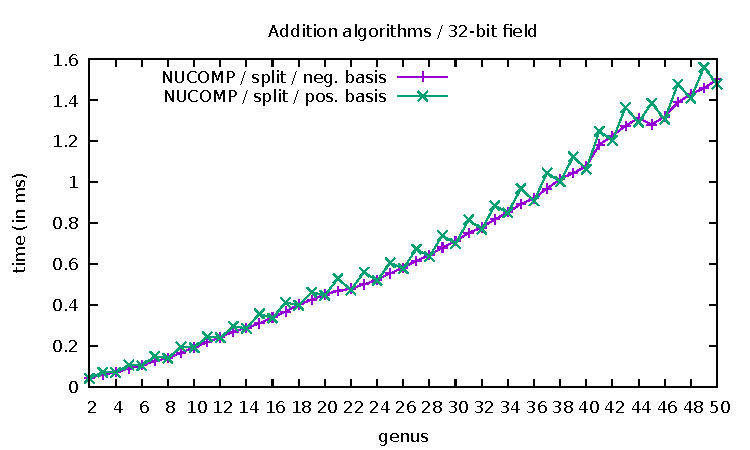
\includegraphics[width=0.775\textwidth]{balNucomp/add_pos_neg_split_32.pdf}}
\centerline{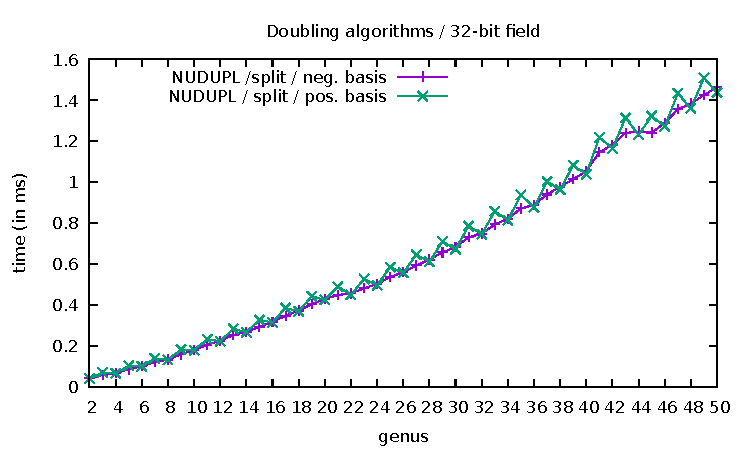
\includegraphics[width=0.775\textwidth]{balNucomp/dbl_pos_neg_split_32.pdf}}

\centerline{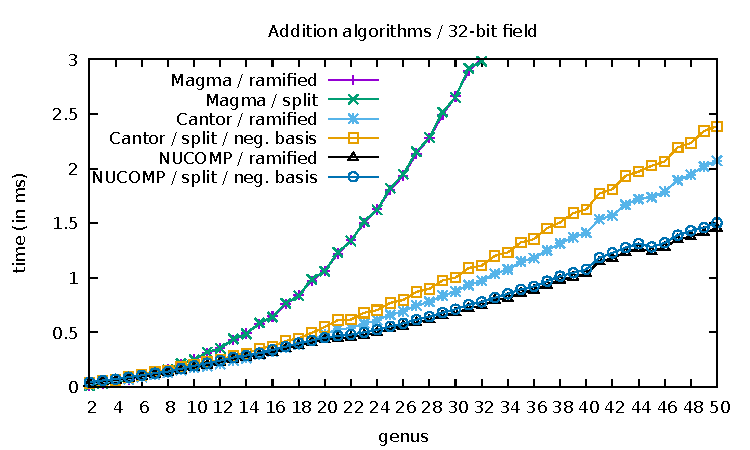
\includegraphics[width=0.775\textwidth]{balNucomp/add_y_32.pdf}}
\centerline{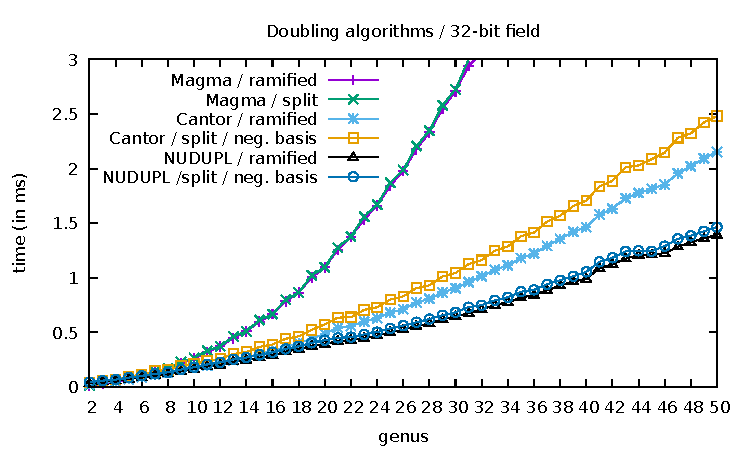
\includegraphics[width=0.775\textwidth]{balNucomp/dbl_y_32.pdf}}

\centerline{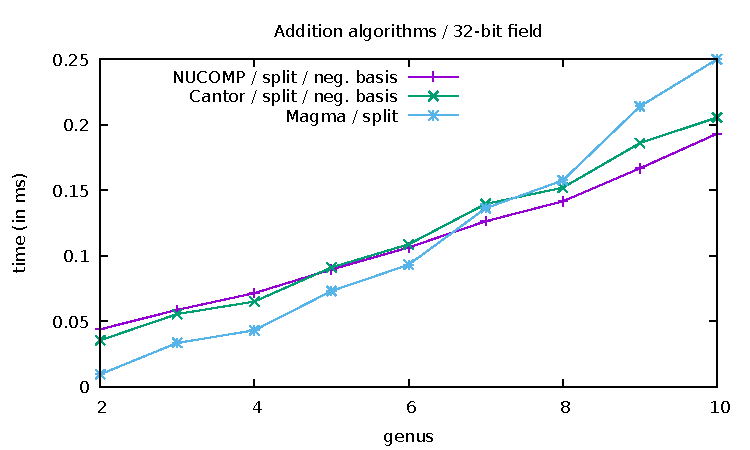
\includegraphics[width=0.775\textwidth]{balNucomp/add_lowg_32.pdf}}
\centerline{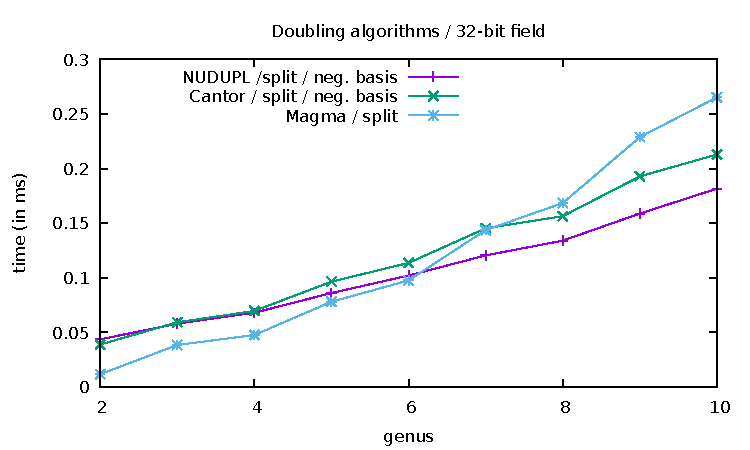
\includegraphics[width=0.775\textwidth]{balNucomp/dbl_lowg_32.pdf}}


The empirical results indicate that Balanced NUCOMP provides an improvement for
computing balanced divisor class arithmetic on hyperelliptic curves given by a
split model with a cross-over as low as genus 5.  As expected, our choice of
normalizing $v$ in negative reduced basis and therefore incorporating
up-adjustments into NUCOMP performs equally well when compared to positive
reduced over even genus, and slightly better over odd. Furthermore, Balanced
NUCOMP performs almost as well and sometimes better than ramified curve NUCOMP
and closes the performance gap between ramified model and split model divisor
arithmetic. 

Improved explicit formulations for divisor arithmetic over split models
in genus 2 and 3 utilize the novel Balanced NUCOMP, and are discussed in
Chapters~\ref{cha:g2} and~\ref{cha:g3}. Moreover, integrating algorithms from
this chapter directly into Magma's built-in arithmetic, or implementing the
algorithms directly in C/C++ so that they do not suffer from the overhead
associated to working in a high-level system like Magma, might reduce the
relative performance, either lowering or elimination any cross-over points
between the algorithms and Magma's arithmetic.

